
% This LaTeX was auto-generated from MATLAB code.
% To make changes, update the MATLAB code and republish this document.

\documentclass{article}
\usepackage{graphicx}
\usepackage{color}

\sloppy
\definecolor{lightgray}{gray}{0.5}
\setlength{\parindent}{0pt}

\begin{document}

    
    

\section*{11. Hermite integral formula}

\begin{verbatim}
ATAPformats
\end{verbatim}
\begin{par}
 If there is a single most valuable mathematical tool in the
analysis of accuracy of polynomial approximations, it is contour integrals in the
complex plane.\footnote{This and the next chapter, together with
Chapter 20, are possibly the
hardest in the book, with a good deal of mathematics presented in a few
pages and heavy use of complex variables.}
From a contour integral one can see why some approximations are
extraordinarily good, like interpolation in Chebyshev points, and
others are impossibly bad, like interpolation in equispaced points. This
chapter presents the basics of the contour integrals, and the next
applies them to take some first steps toward the subject of potential
theory, which relates the accuracy of approximations to equipotential or
minimal-energy problems for electrostatic charge distributions in the
plane. 
\end{par} \vspace{1em}
\begin{par}

The starting ingredients have already appeared in Chapter 5. Following
the formulation there, let $x_0,\dots,x_n$ be a set of $n+1$ distinct
interpolation or ``grid'' points, which may be real or complex, and
define the node polynomial $\ell\in {\cal P}_{n+1}$ as in (5.4) by
$$ \ell(x) = \prod_{k=0}^n (x-x_k) . \eqno (11.1) $$
Repeating (5.5), the function
$$ \ell_j(x) = {\ell(x)\over \ell'(x_j)\kern 1pt (x-x_j)} \eqno (11.2) $$
is the Lagrange polynomial associated with $x_j$, that is, the unique
polynomial in ${\cal P}_n$ that takes the value $1$ at $x_j$ and 0 at the
other points $x_k$.  Following (5.1), a linear combination of these
functions gives the interpolant in ${\cal P}_n$ to an arbitrary function
$f$ defined on the grid:
$$ p(x) = \sum_{j=0}^n f(x_j) \ell_j(x). \eqno (11.3)  $$
\vspace{-1em} 
\end{par} \vspace{1em}
\begin{par}

We now make a crucial observation.  Let $\Gamma_j$ be a contour in the
complex $x$-plane that encloses $x_j$ but none of the other grid points,
nor the point $x$.  (By ``encloses'' we always mean that it winds around
the specified set once in the counterclockwise direction, in the usual
sense of complex variables.)  Then the expression on the right in (11.2)
can be written
$$ {\ell(x)\over \ell'(x_j)\kern 1pt (x-x_j)}
= {1\over 2\pi i} \int_{\Gamma_j}
{\ell(x)\over \ell(t)\kern 1pt (x-t)} \, dt. \eqno (11.4) $$
To verify this formula we ignore the $\ell(x)$ term on both
sides, which has nothing to do with the integral, and use
the fact that $1/(\ell'(x_j) (x-x_j))$ is the {\em residue}
of the function $1/(\ell(t) (x-t))$ at the pole $t=x_j$.

\end{par} \vspace{1em}
\begin{par}

From (11.2) and (11.4) we thus
have an expression for $\ell_j(x)$ as a contour integral:
$$ \ell_j(x)\ = {1\over 2\pi i} \int_{\Gamma_j}
{\ell(x) \over \ell(t) \kern 1pt (x-t)} \, dt, \eqno (11.5) $$
where $\Gamma_j$ encloses $x_j$.  Now let $\Gamma'$ be a contour
that encloses all of the grid points $\{x_j\}$, but still not
the point $x$,
and let $f$ be a function analytic on and interior to
$\Gamma'$.  Then we can combine
together these integrals to get an expression for
the interpolant $p$ to $f$ in $\{x_j\}$:
$$ p(x) = {1\over 2\pi i} \int_{\Gamma'}
{\ell(x) f(t) \over \ell(t) \kern 1pt (x-t)} \, dt. \eqno (11.6) $$
Note how neatly this formula replaces the sum of (11.3) by
a contour integral with contributions from the same points $x_j$.

\end{par} \vspace{1em}
\begin{par}

Now suppose we enlarge the contour of integration to a new contour
$\Gamma$ that encloses $x$ as well as $\{x_j\}$, and we assume $f$ is
analytic on and inside $\Gamma$.  The residue of the integrand of (11.6)
at $t=x$ is $-f(x)$, so this brings in a new contribution $-f(x)$ to the
integral, yielding  an equation for the error in polynomial
interpolation:
$$ p(x) - f(x) = {1\over 2\pi i} \int_\Gamma
{\ell(x) f(t) \over \ell(t) \kern 1pt (x-t)} \, dt. \eqno (11.7) $$ And
thus we have derived one of the most powerful formulas in all of
approximation theory, the {\em Hermite interpolation formula}. This name
comes from Hermite [1878], but the same result had been stated 52 years
earlier by Cauchy [1826]. (Hermite, however, generalized the formulation
significantly to non-distinct or ``confluent'' interpolation points and
corresponding interpolation of derivatives as well as function values;
see Exercise 11.2.)

\end{par} \vspace{1em}
\begin{par}
\textbf{Theorem 11.1.  Hermite interpolation formula.} \textit{Let $f$ be analytic in a region $\Omega$ containing distinct points $x_0,\dots, x_n,$ and let $\Gamma$ be a contour in $\Omega$ enclosing these points in the positive direction.  The polynomial interpolant $p\in {\cal P}_n$ to $f$ at $\{x_j\}$ is}
\end{par} \vspace{1em}
\begin{par}

\vskip -1.5em
$$ p(x) = {1\over 2\pi i} \int_\Gamma
{f(t)\kern 1pt (\ell(t)-\ell(x))\over \ell(t)\kern 1pt (t-x)}
\, dt, \eqno (11.8) $$
\vskip -.5em

\end{par} \vspace{1em}
\begin{par}
\textit{and if $x$ is enclosed by $\Gamma$, the error in the interpolant is}
\end{par} \vspace{1em}
\begin{par}

\vskip -1em
$$ f(x) - p(x) = {1\over 2\pi i} \int_\Gamma
{\ell(x)\over \ell(t)}{f(t)\over (t-x)} \, dt. \eqno (11.9) $$
\vskip -.5em

\end{par} \vspace{1em}
\begin{par}
\textit{Proof.}  Equation (11.9) is the same as (11.7).  For (11.8), we note that if $\Gamma$ encloses $x$, then $f(x)$ can be written $$ f(x) = {1\over 2\pi i} \int_\Gamma {\ell(t)\kern 1pt f(t)\over \ell(t)\kern 1pt (t-x)} \, dt, $$ and combining this with (11.7) gives the result.  But the integrand of (11.8) has no pole at $t=x$, so the same result also applies if $\Gamma$ does not enclose $x$. $~\hbox{\vrule width 2.5pt depth 2.5 pt height 3.5 pt}$
\end{par} \vspace{1em}
\begin{par}
It is perhaps interesting to sketch Cauchy's slightly different derivation from 1826, outlined in $\hbox{[Smithies 1997, p.~117],}$ which may have been influenced by Jacobi's thesis a year earlier [Jacobi 1825]. Cauchy started from the observation that $p(x)/\ell(x)$ is a rational function with denominator degree greater than the numerator degree.  This implies that it must be equal to the sum of the $n+1$ inverse-linear functions $r_j/(x-x_j)$, where $r_j$ is the residue of $p(t)/\ell(t)$ at $t=x_j$ (a partial fraction decomposition, to be discussed further in Chapter 23).  Since $p$ interpolates $f$ at $\{x_j\}$, $r_j$ is also the residue of $f(t)/\ell(t)$ at $t=x_j$.  By residue calculus we therefore have $$ {p(x)\over \ell(x)} = {1\over 2\pi i} \int_{\Gamma'} {f(t)\over \ell(t)\kern 1pt (x-t)}\, dt $$ if $\Gamma'$ is again a contour that encloses the points $\{x_k\}$ but not $x$ itself, or equivalently, (11.6).
\end{par} \vspace{1em}
\begin{par}
Now let us see how Theorem 11.1 can be used to estimate the accuracy of polynomial interpolants.
\end{par} \vspace{1em}
\begin{par}
 Suppose $f$ and $x$ are fixed and we want to estimate $f(x)-p(x)$
for various degrees $n$ and corresponding sets of $n+1$ points $\{x_j\}$.
On a fixed contour $\Gamma$, the quantities $f(t)$ and $t-x$ in (11.9)
are independent of $n$.  The ratio $$ {\ell(x)\over \ell(t)} =
{\prod_{j=0}^n (x-x_j)  \over \prod_{j=0}^n (t-x_j)} ,  \eqno (11.10) $$
however, is another matter.  If $\Gamma$ is far enough from $\{x_j\}$,
then for each $t\in\Gamma$, this ratio will shrink exponentially as
$n\to\infty$, and if this happens, we may conclude from (11.9) that
$p(x)$ converges exponentially to $f(x)$ as $n\to\infty$. The crucial
condition for this argument is that it must be possible for $f$
to be analytically continued as far out as $\Gamma$. 
\end{par} \vspace{1em}
\begin{par}
Here is a warm-up example mentioned in $\hbox{[Gaier 1987, p. 63]. }$ Suppose the interpolation points $\{x_j\}$ lie in $[-1,1]$ for each $n$ and $x\in[-1,1]$ also.  Let $S$ be the ``stadium'' in the complex plane consisting of all numbers lying at a distance $\le 2$ from $[-1,1]$, and suppose $f$ is analytic in a larger region $\Omega$ that includes a contour $\Gamma$ enclosing $S$.  We can sketch the situation like this:
\end{par} \vspace{1em}
\begin{par}
 \vspace{-2em} 
\end{par} \vspace{1em}
\begin{verbatim}
x = chebfun('x');
hold off, plot(real(x),imag(x),'r')
semi = 2*exp(0.5i*pi*x);
S = join(x-2i, 1+semi, 2i-x, -1-semi);
hold on, plot(S,'k'), axis equal off
z = exp(1i*pi*x);
Gamma = (2.8+.2i)*(sinh(z)+.5*real(z));
plot(Gamma,'b')
text(4.2,2,'\Gamma','color','b','fontsize',12)
text(3.1,.7,'S','fontsize',12)
text(.9,-.3,'1','color','r')
text(-1.4,-.3,'-1','color','r')
\end{verbatim}

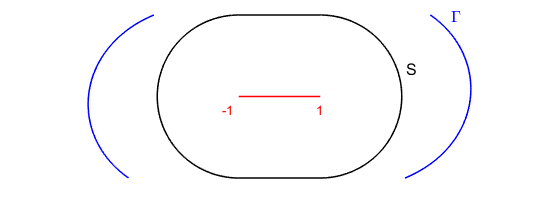
\includegraphics [width=4in]{chap11_01.png}
\begin{par}
Under these assumptions, there is a constant $\gamma>1$ such that for every $t\in \Gamma$ and every $x_j$, $|t-x_j| \ge \gamma |x-x_j|$.  This implies, $$ |\ell(x)/\ell(t)| \le \gamma^{-n-1} $$ and thus by (11.9), $$ \|f-p\| = O(\gamma^{-n}). $$ Note that this conclusion applies regardless of the distribution of the interpolation points in $[-1,1]$. They could be equally spaced or random, for example.  (At least that is true in theory.  In practice, such choices would be undone by rounding errors on a computer, as we shall see in the next chapter.)
\end{par} \vspace{1em}
\begin{par}
So convergence of polynomial interpolants to analytic functions on $[-1,1]$ is all about how small $\ell(x)$ is on $[-1,1]$, compared with how big it is on a contour $\Gamma$ inside which $f$ is analytic.  From this point of view we can begin to see why Chebyshev points are so good: because a polynomial with roots at the Chebyshev points has approximately uniform magnitude on $[-1,1]$. Suppose for example we consider the polynomial $\ell\in {\cal P}_8$ with roots at 8 Chebyshev points.  On $[-1,1]$ it has size $O(2^{-8})$, roughly speaking, but it grows rapidly for $x$ outside this interval.  Here is a plot for $x \in [-1.5,1.5]$:
\end{par} \vspace{1em}
\begin{par}
 \vspace{-2em} 
\end{par} \vspace{1em}
\begin{verbatim}
np = 8; xj = chebpts(np); FS = 'fontsize';
d = domain(-1.5,1.5);
ell = poly(xj,d);
hold off, plot(ell), grid on
hold on, plot(xj,ell(xj),'.k'), ylim([-.5 1.5])
title('A degree 8 polynomial with roots at Chebyshev points',FS,9)
\end{verbatim}

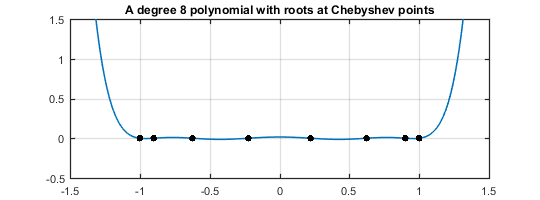
\includegraphics [width=4in]{chap11_02.png}
\begin{par}
 \vspace{1pt} 
\end{par} \vspace{1em}
\begin{par}
With Matlab's \texttt{contour} command we can examine the size of $\ell(x)$ for complex values of $x$. The following code plots contours at $|\ell(x)| = 2^{-6}, 2^{-5},\dots,1.$
\end{par} \vspace{1em}
\begin{par}
 \vspace{-2em} 
\end{par} \vspace{1em}
\begin{verbatim}
hold off, plot(xj,ell(xj),'.k','markersize',10)
hold on, ylim([-0.9,0.9]), axis equal
xgrid = -1.5:.02:1.5; ygrid = -0.9:.02:0.9;
[xx,yy] = meshgrid(xgrid,ygrid); zz = xx+1i*yy;
ellzz = ell(zz); levels = 2.^(-6:0);
contour(xx,yy,abs(ellzz),levels,'k')
title(['Curves |l(x)| = 2^{-6}, 2^{-5}, ..., 1 '...
    'for the same polynomial'],FS,9)
\end{verbatim}

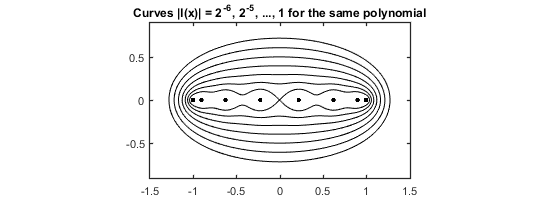
\includegraphics [width=4in]{chap11_03.png}
\begin{par}
 \vspace{1pt} 
\end{par} \vspace{1em}
\begin{par}
We can see a great deal in this figure.  On $[-1,1]$, it confirms that $\ell(x)$ is small, with maximum value $|\ell(x)| = 2^{-6}$ at $x=0$. Away from $[-1,1]$, $|\ell(x)|$ grows rapidly and takes constant values on curves that look close to ellipses.  For $t$ on the outermost of the curves plotted, the ratio $|\ell(x)/\ell(t)|$ will be bounded by $2^{-6}$ for any $x\in[-1,1]$.
\end{par} \vspace{1em}
\begin{par}
Let us compare this to the very different behavior if we take points that are not close to the Chebyshev distribution. To make a specific and quite arbitrary choice, let us again take 8 points, four of them at $-1$ and four at $1$.  Here is the plot on the real axis.
\end{par} \vspace{1em}
\begin{par}
 \vspace{-2em} 
\end{par} \vspace{1em}
\begin{verbatim}
xj = [-1 -1 -1 -1 1 1 1 1];
ell = poly(xj,d);
hold off, plot(ell), grid on
hold on, plot(xj,ell(xj),'.k'), ylim([-.5 1.5])
title('A degree 8 polynomial with roots at 1 and -1',FS,9)
\end{verbatim}

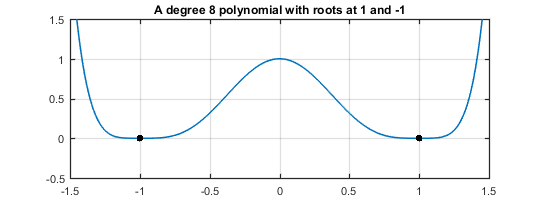
\includegraphics [width=4in]{chap11_04.png}
\begin{par}
 \vspace{1pt} 
\end{par} \vspace{1em}
\begin{par}
And here are the contours in the complex plane.
\end{par} \vspace{1em}
\begin{par}
 \vspace{-2em} 
\end{par} \vspace{1em}
\begin{verbatim}
hold off, plot(xj,ell(xj),'.k'), hold on
ylim([-0.8,0.8]), axis equal, ellzz = ell(zz);
contour(xgrid,ygrid,abs(ellzz),levels,'k')
title(['Curves |l(x)| = 2^{-6}, 2^{-5}, ..., 1 '...
    'for the same polynomial'],FS,9)
\end{verbatim}

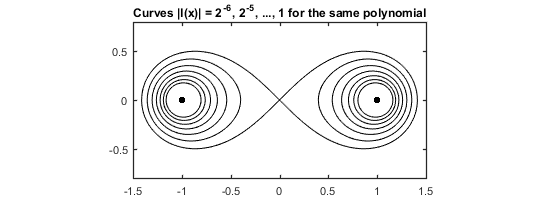
\includegraphics [width=4in]{chap11_05.png}
\begin{par}
 \vspace{1pt} 
\end{par} \vspace{1em}
\begin{par}
These figures show that the size of $\ell(x)$ on $[-1,1]$ is not at all uniform: it is far smaller than $2^{-6}$ for $x\approx \pm 1$, but as big as $1$ at $x=0$.  Now, for $x\in [-1,1]$ and $t$ on the outermost curve shown, the maximum of the ratio $|\ell(x)/\ell(t)|$ is no better than $1$ since that curve touches $[-1,1]$. If we wanted to achieve $|\ell(x)/\ell(t)| \le 2^{-6}$ as in the last example, $\Gamma$ would have to be a much bigger curve---closer to the ``stadium'':
\end{par} \vspace{1em}
\begin{par}
 \vspace{-2em} 
\end{par} \vspace{1em}
\begin{verbatim}
xgrid = -2:.04:2; ygrid = -1.5:.04:1.5;
[xx,yy] = meshgrid(xgrid,ygrid); zz = xx+1i*yy;
ellzz = ell(zz); levels = 2.^(-6:0); levels = [2^6,2^6];
hold on, contour(xgrid,ygrid,abs(ellzz),levels,'r')
ylim([-1.5 1.5]), axis equal
title('Another contour added at level 2^6',FS,9)
\end{verbatim}

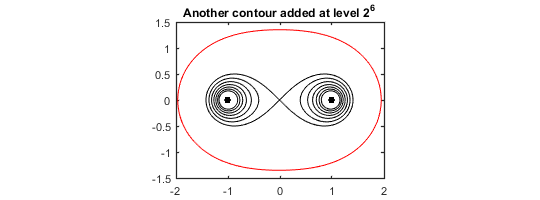
\includegraphics [width=4in]{chap11_06.png}
\begin{par}
 \vspace{1pt} 
\end{par} \vspace{1em}
\begin{par}
The function $f$ would have to be analytic within this much larger region for the bound (11.9) to apply with a ratio $|\ell(x)/\ell(t)|$ as favorable as $2^{-6}$.
\end{par} \vspace{1em}
\begin{par}

\begin{displaymath}
\framebox[4.7in][c]{\parbox{4.5in}{\vspace{2pt}\sl
{\sc Summary of Chapter 11.}
The error of a polynomial interpolant can be represented by a contour
integral in the complex plane, the Hermite integral formula.  This
provides the standard method for showing geometric convergence for
certain approximations of analytic functions.\vspace{2pt}}}
\end{displaymath}

\end{par} \vspace{1em}
\begin{par}
 \small\smallskip\parskip=2pt
{\bf Exercise 11.1.  Chebfun computation of Cauchy integrals.}
(a) Figure out (on paper) the polynomial $p\in {\cal P}_2$ that takes the
values $p(-1) = 1$, $p(1/2) = 2$, and $p(1)=2$. What is $p(2)$?
(b) Read about the numerical computation of Cauchy integrals in Chapter 5
of the online {\em Chebfun Guide}.  Write a program to confirm Theorem
11.1 by computing $p(2)$ numerically by a Cauchy integral for the
function $f(x) = (x+1)(x-0.5)(x-1)e^x + 11/6 + x/2 - x^2/3$. Take both
$|x| = 3/2$ and $|x| = 3$ as contours to confirm that it does not matter
whether or not $\Gamma$ encloses $x$.
(c) Write an anonymous function \verb|p = @(x) ...| to apply the above
calculation not just for $x=2$ but for arbitrary $x$, and construct a
chebfun on $[-1,1]$ from this anonymous function. Do its coefficients as
reported by {\tt poly} match your expectations?
\par
{\bf Exercise 11.2.  Confluent interpolation points.} Modify the above
problem to require $p(-1) = 1$, $p(1) = 2$, and $p'(1) = 0$.  This is a
{\em Hermite interpolation problem,} in which some interpolation points
are specified multiply with corresponding values specified for
derivatives.  What is the analytic solution to this interpolation
problem?  Do the computations involving contour integrals and anonymous
functions deliver the right result?
\par
{\bf Exercise 11.3.  Interpolation in a disk.}
Suppose a function $f$ is interpolated by polynomials in arbitrary points
of the disk $|x|\le r'$ and we measure the accuracy $f(x)-p(x)$ for $x$
in the disk $|x|\le r$.  Show that geometric convergence is assured (in
exact arithmetic, ignoring rounding errors) if $f$ is analytic in the
disk $|x| \le r+2r'$. Give the constant $\rho$ for convergence at the
rate $O(\rho^{-n})$. (This result originates with [M\'eray 1884].)
\par
{\bf Exercise 11.4.  Working around a simple pole.}
Let $f$ be analytic on the closed Bernstein ellipse region
$\overline E_\rho$ for some $\rho>1$.  It can be shown that
$|\ell(x)/\ell(t)| = O(\kern.5pt \rho^{-n})$ uniformly as $n\to\infty$ for
$x\in [-1,1]$ and $t$ on the ellipse, and thus Theorem 11.1 can be
used to show that $\|f-p_n\|=O(\kern .5pt\rho^{-n})$ as asserted by
Theorem~8.2.
Now suppose that $f$ has one or more singularities on the ellipse
but these are just simple poles.  Explain how the contour integral
argument can be modified to show that the rate of convergence
will still be $\|f-p_n\|=O(\kern .5pt\rho^{-n})$, as was established
by another method in Exercise 8.15.

\end{par} \vspace{1em}



\end{document}
    
